\documentclass[8pt]{article}

\title {\textbf{Vulkan Renderer}}
\date{June 2022}

\usepackage{blindtext}
\usepackage{amsmath}
\usepackage{multicol}
\usepackage{geometry}
\usepackage{hyperref}
\usepackage{graphicx}

\geometry{
	a4paper,
	left=20mm,
	%right=
	%bottom=
	top=15mm}

\begin{document}
		\maketitle

		\begin{figure}[h!]
			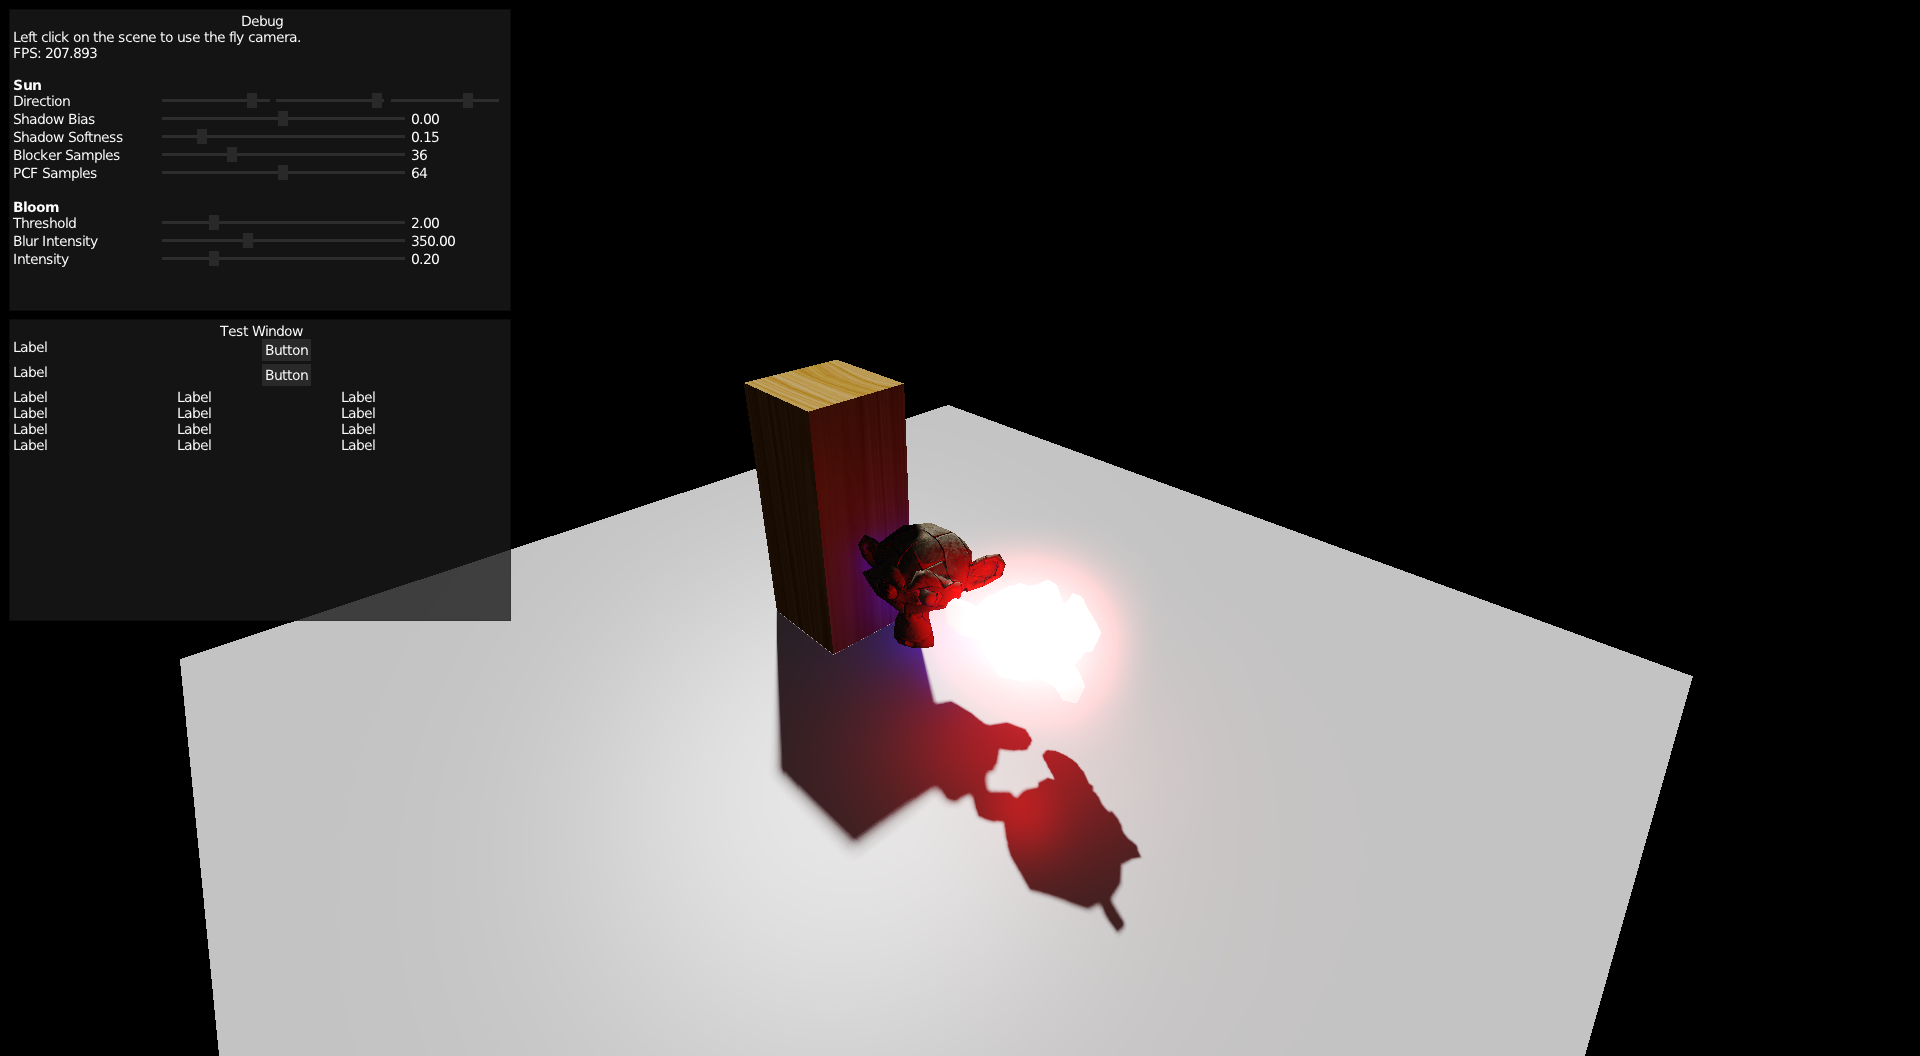
\includegraphics[width=\linewidth]{media/screenshot_001.png}
			\caption{PCSS makes the shadow appear more or less soft depending on the distance of the blocker.}
			\label{fig:pcss}
		\end{figure}

		\begin{multicols}{2}
			\section{Brief}
			The modular system is to be a real-time 3-D renderer that makes
			use of the Vulkan API. It will include the following features:
			 - Wavefront loading.
			 - 3-D lighting including normal mapping and soft shadows.
			 - Simple post-processing effects such as Bloom.

			It will rely on GLFW for windowing and input. The rest is to be
			implemented from scratch in C++.

			The renderer will be built as a dynamic library/shared object, to
			be linked to a client application. This is so that any external
			libraries that the renderer relies on won't have to be linked into
			client applications as well, which would be the case if the renderer
			were linked to clients statically.

			The renderer will make use of various mathematical functions for
			3-D transformation including vector operations such as the dot
			and cross product and matrix operations like translation, rotation,
			scaling and projection matrices. It will also provide soft shadows
			using PCSS and PCF.

			The renderer will provide a base class for applications that clients
			inherit from which provides functionality like abstracting the GLFW
			windowing and input, as well as creating the Vulkan instance. The
			goal is for all Vulkan calls to be abstracted behind at least a thin
			object-oriented layer. For example, a "Mesh" class which will manage
			vertex and index buffers for the user that they can simply push data
			into and draw on command, or a "Scene" class that manages different
			meshes, post processing effects and lights.

			\section{Implementation Overview}
			The final features include:
			\begin{itemize}
				\item Wavefront loader.
				\item 3-D rendering, point lighting and normal mapping using deferred shading.
				\item Percentage-Closer Soft Shadows.
				\item Bloom and tone mapping.
				\item Vulkan API abstraction.
				\item Basic GUI.
				\item 2-D rendering using texture atlasing.
			\end{itemize}

			The Vulkan API abstraction creates and object-oriented layer around
			textures and buffers (vertex, index and frame buffers), GLFW windows,
			as well as the graphics pipeline. The Renderer3D and Renderer2D classes
			build abstractions on top of the API abstraction to provide extra
			functionality and provide an easy-to-use layer that allows easy rendering
			of 3-D objects and 2-D sprites.

			The 2-D rendering uses a texture atlasing system that packs all of the
			textures that it requires on the fly, so that the shader only ever has
			to sample a single texture. The algorithm it uses to do this is extremely
			stupid and simply lines up all of the textures along the x axis.

			The shadow mapping makes use of a technique named "Percentage-Closer
			Shadow Mapping" (PCSS). This technique samples the depth map in terms of
			the surface to gain an average of how far away the shadow blockers are
			(the "blocker search"). Using that average, it uses a formula described in
			\href{https://developer.download.nvidia.com/shaderlibrary/docs/shadow_PCSS.pdf}{this paper} 
			to estimate the size of the penumbra of the shadow. Then, the shader runs
			a PCF algorithm on the shadow map with a radius that depends on the
			penumbra size. This has the effect of causing the shadow to appear
			more soft the further away the object blocking the light is from the
			surface that's receiving the shadow. This is particularly visible in
			Figure \ref{fig:pcss}.

			\section{Performance Evaluation}
			The 3-D renderer's performance is real-time but not brilliant compared
			to the renderers included in tools such as Unity. This is mostly due
			to the low speed of some of the post processing effects, namely Bloom,
			which samples the texture quite heavily. The shadow-mapping uses PCF,
			which requires a lot of samples to avoid unwanted effects such as
			banding. Another technique that might improve speed would be Variance
			shadow mapping, though that would greatly increase the complexity of
			the system should PCSS also be desired, probably requiring the use of
			a compute shader. With bloom and soft-shadows enabled using 36 samples
			for the shadow blocker search and 64 samples PCF, the renderer can run
			at between 200 and 300 FPS on my Radeon RX 570 GPU, running an optimised
			and stripped build.
		\end{multicols}
\end{document}
